\documentclass[
ngerman,
%english,
cdfont=true,
abstract=section,
BCOR=4mm]{tudscrreprt}

\iftutex
  \usepackage{fontspec}
\else
  \usepackage[T1]{fontenc}
  \usepackage[ngerman=ngerman-x-latest]{hyphsubst}
\fi
\usepackage{babel}
\usepackage{isodate}
\usepackage{pdfpages}
\usepackage{tabularx}
\usepackage{listings}
\usepackage{color}
\definecolor{dkgreen}{rgb}{0,0.6,0}
\definecolor{gray}{rgb}{0.5,0.5,0.5}
\definecolor{mauve}{rgb}{0.58,0,0.82}

\lstset{frame=tb,
  language=Python,
  aboveskip=3mm,
  belowskip=3mm,
  showstringspaces=false,
  columns=flexible,
  basicstyle={\small\ttfamily},
  numbers=none,
  numberstyle=\tiny\color{gray},
  keywordstyle=\color{blue},
  commentstyle=\color{dkgreen},
  stringstyle=\color{mauve},
  breaklines=true,
  breakatwhitespace=true,
  tabsize=3
} 

\usepackage[unicode=true,
 bookmarks=true,bookmarksnumbered=false,bookmarksopen=true,bookmarksopenlevel=1,
 breaklinks=false,pdfborder={0 0 0},backref=false,colorlinks=false]
 {hyperref}
\usepackage{graphicx}
\usepackage[thinlines]{easytable}
\graphicspath{ {./images/} }
\newcommand{\myminted}[1]{\inputminted{python}{scripts/#1}}
 

%
% Paket fr Links innerhalb des PDF Dokuments
%
\definecolor{LinkColor}{rgb}{0,0,0.5}
\usepackage[all]{hypcap}
\usepackage{hypbmsec}

\newcommand {\ThesisTitle}{Thesis title}
\newcommand {\AuthorName}{Student name}
\newcommand {\ThesisType}{Bachelor thesis}
\newcommand {\SupervisorName}{Supervisor name}


%
% Metainformationen für das zu erzeugende PDF
%
\hypersetup{
 pdftitle={\ThesisTitle},
 pdfauthor={\AuthorName},
 pdfsubject={\ThesisType}}

\usepackage[style=numeric]{biblatex}
\addbibresource{articles.bib}
\begin{document}
\faculty{Faculty of Computer Science}
\institute{Institute of Systems Architecture}
\chair{Chair of Privacy and Data Security}
\date{}
\title{%
   \ThesisTitle
}
\subject{bachelor}
\graduation[B.Sc]{Bachelor of Science}
\author{%
  \AuthorName
  \matriculationnumber{4803900}%
  \dateofbirth{25.12.1999}%
  \placeofbirth{Dresden}%
}
\matriculationyear{2018}
\supervisor{Supervisor}
\professor{Prof. Dr. Professor}

\maketitle

% include task description

\includepdf{Aufgabenstellung.pdf}
\cleardoublepage
\confirmation[\SupervisorName]

\begin{abstract}
Um den Betrieb der Computernetzwerke unserer Zeit zu gewährleisten, ist es von äußerster Wichtigkeit, möglichst alle Angriffe und bösartigen Netzwerkverkehr zu erkennen, ohne dabei den menschlichen Administrator hinter dem System zu überfordern. Diese Tatsache macht Monitoring und damit Intrusion Detection Systeme zu einem Grundpfeiler einer jeden Strategie der Netzwerksicherheit. Etablierte Implementierungen müssen dabei stetig an sich ändernde äußere Umstände angepasst werden. Einer der zentralen Ansätze, um die Anpassungsfähigkeit gängiger Netzwerkssicherheitskomponenten möglichst ohne menschliches Zutun zu erhöhen oder überhaupt erst zu schaffen, ist Kontextsensitivität, also die Verwendung von Kontext, um dem relevanten Informationen und/oder Dienstleistungen bereitzustellen. In dieser Arbeit wurde diskutiert, wie Kontextinformationen kategorisiert, akquiriert und geformt werden können. Mithilfe des Kontextes wurde die Leistung von Zeek, einem hybriden kontextsensitiven IDS, verbessert und abschließend aufbauend darauf ein Urteil über die einzelnen Kategorien und deren Nützlichkeit zur Erhöhung der Sicherheit abgegeben.
\end{abstract}


\newpage{}
\tableofcontents{}
\newpage{}



%
\chapter{General notes}%
\label{cha:general_notes}

This chapter is not part of the typical outline of written thesises and only serves the purpose of providing more general advice that is not specific to any of the following chapters.

\begin{itemize}
\item Citations can be done using the cite command. It is possible to place multiple references in the cite command, e.g. %\cite{zobel2004writing,booth2003craft}.
\item In general, it might not be the best approach to write the texts of the chapters in the same order as the chapters appear (e.g. first write introduction, then background, and so on. Instead, you can also consider to start writing the introduction chapter first to check how good your understanding of your own contribution is, as during writing, you are likely to discover gaps in your argumentation or implicit assumptions that you made.
\item To get into writing mode, you may just start to write down your thoughts freely first without being to critical about your argumentation, grammar and so on and incrementally improve your text. 
\item When you write your thesis or any other scientific text, it is recommended that you think about what the target audience of your work is and following from that, what you can assume about their prior knowledge.
When it comes to a thesis, you should assume the reader to have the same knowledge about the topic as your fellow students may have.
\end{itemize}

\chapter{Einführung}
\label{cha:introduction}

%The introduction serves the purpose of educating the reader about the broader context or research problem that your work addresses and its relevance as well as the relevance of your work towards solving this problem.
%As a rough guideline, this section should be written to answer the following questions:
%\begin{enumerate}
%   \item What is the problem your work addresses?
%   \item Why is it desirable to solve this problem? (e.g. which new possibilities/use cases become possible if the problem is solved)
 %  \item Roughly, what contribution towards solving the problem will you present to the reader in this thesis?
%\end{enumerate}

Seit Computernetzwerke existieren, gibt es auch Menschen, welche sich zu diesen widerrechtlichen Zugang verschaffen wollen. Weder Sicherheitsmaßnahmen noch deren Weiterentwicklung haben diesen Umstand bisher geändert. Lediglich die Netzwerke, welche dabei von Interesse sind, haben sich gewandelt und stellen die IT-Sicherheit dabei immer wieder vor neue Herausforderungen, die zunehmend nicht mehr ausschließlich manuell gelöst werden können. Gleichzeitig verändern sich auch Angreifer und ihre Angriffsarten und die dabei verwendeten Werkzeuge und Techniken entwickeln sich weiter und ermöglichen nach wie vor, in kontrollierte Umgebungen einzudringen, Schäden zu verursachen und dabei trotzdem unentdeckt zu bleiben. Dagegen stehen einem Netzwerkadministrator allerdings eine Vielzahl von Mitteln zur Verfügung. Unter anderem Netzwerk-Sicherheits-Monitoring, dessen erste Stufe beim Umgang mit Angriffen die Erkennung darstellt. Etabliert hat sich dabei vor allem die Verwendung von Intrusion Detection Systemen, welche aber wie jedes System dieses Komplexitätsgrades nie gänzlich fehlerfrei arbeiten. Deshalb ist es letztendlich immer noch nötig, dass die Entscheidungen eines IDS regelmäßig durch einen Menschen überprüft und gegebenenfalls korrigiert werden. Um also die Menge an Meldungen, welche manuell überprüft werden müssen, zu verringern und die Aussagekraft der erzeugten Alarme zu erhöhen und damit den menschlichen Entscheider zu entlasten sowie generell seine Aufgaben besser zu erfüllen, muss ein IDS eine möglichst große Zahl von Szenarien korrekt einschätzen. Dazu werden Informationen benötigt, mit denen die Geschehnisse in einem Netzwerk in einer für das IDS verständlichen Form vollständig abgebildet werden können. In dieser Arbeit soll ergründet werden, wie diese Ziele mit Kontextsensitivität erfüllbar sind und welche Art von Kontext dafür am besten geeignet ist.
\chapter{Hintergrund}%
\label{cha:background}

%The background chapter aims to give a more detailed introduction into the context of your work and provides additional information that enables the target audience to understand the argumentations and motivations that you explain in the following chapters.
%This chapter is typically read on demand, if in the following chapters, the reader encounters a term or argumentation that is not immediately clear from the corresponding chapter alone.


%\subsection{Angreifermodell}

%\paragraph{Kontextsensitivität}
%“A system is context-aware if it uses context to provide relevant information and/or services to the user, where relevancy depends on the user’s task.” 

%Ein System ist kontextsensitiv wenn es Kontext verwendet um dem Nutzer mit für ihn relevanten Informationen und/oder Dienstleistungen zu versorgen. Die Relevanz hängt dabei von der Aufgabe des Nutzers ab \cite{dey_understanding_2001}.
%\paragraph{Situation}
%“As defined by Endsley [76], the situation comprises the perception of the elements in the environment within a volume of time and space, the comprehension of their meaning, and the projection of their status in the near future.” 
%Eine Situation 
%TODO
%\paragraph{Umgebung}
%Environment is a synonym for context and does not add to our investigation of context.
%\cite{abowd_towards_1999}
%Umgebung ist ein Synonym für Kontext \cite{abowd_towards_1999}.
%TODO

%\paragraph{Policy}
%TODO
\section{Netzwerk-Sicherheits-Monitoring}
Ghafir et al. \cite{ghafir_network_2015} beschreiben Sicherheits-Monitoring und dessen Aufgaben als eine Reihe von Mechanismen, die ermöglichen, den momentanen Zustand und langfristige Trends eines komplexen Computernetzwerks zu erkennen. Netzwerküberwachung umfasst mehrere Methoden, die gezielt eingesetzt werden, um die Sicherheit und Zuverlässigkeit aufrechtzuerhalten. Dabei reicht das Aufgabenfeld von Hardware, Software, Viren, Spyware und Schwachstellen wie Hintertüren bis zu Sicherheitslücken sowie anderen Aspekten, die die Integrität eines Netzwerks gefährden können. Um proaktiv statt reaktiv vorgehen zu können, muss der Datenverkehr und die Leistung im gesamten Netzwerk überwacht werden, um sicherzustellen zu können, dass keine Sicherheitslücken im Netzwerk auftreten. Im Falle eines Netzwerkfehlers müssen Fehlfunktionen erkannt, isoliert und behoben werden. Bei einem stabilen Netz ist ständige Überwachung, ob eine Bedrohung von innerhalb oder außerhalb vorliegt, notwendig.
\subsection{Intrusion Detection}
Scarfone et al. \cite{scarfone2007guide} erklären Angriffserkennung, als Prozess der Überwachung von Ereignissen in einem Computersystem oder Netzwerk und die Analyse dieser Ereignisse auf Anzeichen eines möglichen Zwischenfalls. Gemeint sind damit Verstöße oder unmittelbare Bedrohungen von Sicherheitsrichtlinien, Akzeptanzrichtlinien oder Standardsicherheitspraktiken.
\subsection{Intrusion Detection System (IDS)}
Aufbauend auf der Definition von Intrusion Detection bezeichnen die Autoren ein IDS somit Software, die den Prozess, einen Eingriff zu erkennen, automatisiert \cite{scarfone2007guide}.
Nach Jones et al. \cite{jones_computer_nodate} werden Informationssysteme immer umfassender werden und haben einen stetig höher werdenden Wert für Netzwerksicherheit. 
Schneier \cite{schneier_managed_2001} bezeichnet IDS vereinfacht als das Netzwerkäquivalent zu Virenscannern. IDS untersuchen den Netzwerkverkehr oder die auf den Hosts laufenden Prozesse auf Anzeichen für einen Angriff. Wenn sie einen solchen erkennen, schlagen sie Alarm. Seiner Ansicht nach sind IDS dabei nicht darauf ausgelegt, dass jeder Angriff identifiziert wird. Da es immer ein Angriffsszenario gibt, in dem ein ausreichend geschickter Angreifer ein Erkennungssystem umgehen können wird. Trotzdem stellt ein IDS eine wirksame Sicherheitsmaßnahme als Teil der Detektionsphase von NSM dar.
%Management of networking requires monitoring. Network monitoring is a set of mechanisms that allows network administrators to know instantaneous state and long-term trends of a complex computer network. Network Monitoring involves multiple methods which are deployed on purpose to maintain the security and integrity of an internal network. monitoring encompasses hardware, software, viruses, spyware, vulnerabilities such as backdoors and security holes, and other aspects that can compromise the integrity of a network. Network monitoring is a difficult and demanding task that is a vital part of a network administrators job. In order to be proactive rather than reactive,administrators need to monitor traffic movement and performance throughout the network and verify that security breaches do not occur within the network. When a network failure occurs, monitoring agents have to detect, isolate, and correct malfunctions in the network and possibly recover the failure. With the stable network, the administrators' jobs remain to monitor constantly if there is a threat from either inside or outside network. 

%intrusion detection is “the process of monitoring the events occurring in a computer system or network and analyzing them for signs of possible incidents, which are violations or imminent threats of violation of computer security policies, acceptable use policies, or standard security practices.”
%When a user of an information system takes an action that that user was not legally allowed to take, it is called intrusion. The intruder may come from outside, or the intruder may be an insider, who exceeds his limited authority to take action. Whether or not the action is detrimental, it is of concern because it might be detrimental to the health of the system, or to the service provided by the s
% As information systems have come to be more comprehensive and a higher value asset of organizations, complex, intrusion detection subsystems have been incorporated as elements of operating systems, although not typically applications. Most intrusion detection systems attempt to detect suspected intrusion, and then they alert a system administrator.
% Given the preceding definition, an IDS can be seen as the software that automates the intrusion detection process.
%IDSs are the network equivalent of virus scanners. IDSs look at network traffic, or processes running on hosts, for signs of attack. If they see one, they sound an alarm. 
%I think of IDSs as network sensors, similar to a burglar alarm on a house. It won’t detect every attack against the house, it can be bypassed by a sufficiently skilled burglar, but it is an effective security countermeasure.
\chapter{Voraussetzungen und verwandete Arbeiten}
\label{cha:requirements_and_related_work}

%In this section, you should point out which requirements a good solution to the problem addressed in your thesis should fulfill.
%It makes sense to state functional as well as non-functional requirements.

%When it comes to the related work, you should then point out to which extent the existing works / proposed solutions already fulfill the requirements you introduced previously.


\subsection{Kontextsensitivität}
%“A system is context-aware if it uses context to provide relevant information and/or services to the user, where relevancy depends on the user’s task.” 

Ein System ist kontextsensitiv wenn es Kontext verwendet um dem Nutzer mit für ihn relevanten Informationen und/oder Dienstleistungen zu versorgen. Die Relevanz hängt dabei von der Aufgabe des Nutzers ab.
\chapter{Design}%
\label{cha:design}

%In this chapter, you should present your solution in detail but at a conceptual level. This means that you explain the overall design including your motivation for this design but you do not provide details on the actual implementation of your design (e.g., in which programming language you wrote it, how the software is structured and so on). This means that you should also point out the aspects where you had different design options and in which points they differ. A good approach to write this chapter is to make yourself aware of the different aspects and design problems that need to be addressed in your design. To do so, you can then proceed repeatedly in three steps:
%\begin{enumerate}
 %  \item Explain a design problem that needs to addressed by the solution (e.g. to enable anonymous communication over the internet, participants need to be able to send messages to each other without revealing identifying to the corresponding receiver).
  % \item Discussion of design choices (e.g. Mix Networks, DC-Networks, etc.) with regards to the requirements from the previous chapter and identification of the most promising choices.
%\end{enumerate}
%After the second step, you start the next iteration by identifying design problems that arise when you want to use the most promising design choice. For example, if Mix networks turn out to be the most promising approach for your requirements, you then need to address the question how the mix network should be designed (e.g. how are mix nodes chosen by the users of the anonymization network? How do mix nodes process messages?). Once you identified the most promising solutions to that, you can then start the next iteration and so on until there are no more open design questions that you are aware of.
Zuerst erläutere ich die meiner Meinung nach bestehende Notwendigkeit für eine Taxonomie. Dann definiere ich die Kontextkategorien meiner Taxonomie. Danach definiere ich in welcher Form die Kontextinformationen in den einzelnen Kategorien vorliegen müssen und wie man Informationen aus unterschiedlichen Quellen in einer für IDS-Signaturen verwendbaren Form gewinnt. Zusätzlich gehe ich noch darauf ein welchen Anforderungen ich an ein IDS stelle und welche Schwächen ich in dem von mir gewählten IDS mithilfe von Kontextsensitivität lösen will. Abschließend bewerte ich wie gut sich die benötigten Kontextinformationen gewinnen lassen. 

\section{Notwendigkeit einer Taxonomie}
%TODO “Based on the evaluation of context categorisation, it is evident that no single categorisation scheme can accommodate all the demands” ([Perera et al., 2014, p. 423]
Die Evaluation verschiedener Kategorisierungsschemata zeigt das keine Kategorisierung allen Ansprüchen gerecht werden kann\cite{perera_context_2014}.
\section{ Erstellung einer Kontexttaxonomie }
Im folgenden möchte ich meinen Versuch einer Kombination der bereits vorgeschlagenen Kategorisierungsschemata erläutern. Dazu lege ich zuerst die Definition der einzelnen Kategorien im Bezug auf kontextsensitive Zugriffskontrolle fest. Die Kategorien müssen dafür, abhängig davon mit welchem Fokus sie der jeweilige Autor konstruiert hat, mehr oder weniger stark angepasst werden.
\subsection{Konzeptionell}
Einordnung anhand der Bedeutung des Kontextes und der begrifflichen Beziehungen.
\subsubsection{Primär}
%“Any information retrieved without using existing context and without performing any kind of sensor data fusion operations (e.g. GPS sensor readings as location information).” 
Kontextinformationen die gesammelt werden können ohne bereits vorhandene Daten zu verwenden oder zu kombinieren. \cite{abowd_towards_1999}
\subsubsection{Sekundär}
%"Any information that can be computed using primary context. The secondary context can be computed by using sensor data fusion operations or data retrieval operations such as web service calls (e.g. identify the distance between two sensors by applying sensor data fusion operations on two raw GPS sensor values). Further, retrieved context such as phone numbers, addresses, email addresses, birthdays, list of friends from a contact information provider based on a personal identity as the primary context can also be identified as secondary context.” 
Kontext der durch das verarbeiten von primärem Kontext erschlossen werden kann. Dies kann durch die Kombination einzelner Datenpunkte einer oder mehrerer Kategorien oder durch Abfragen weiterer Informationen mithilfe der primären Informationen geschehen \cite{abowd_towards_1999}.
\subsection{Betrieblich}
Wie schon in der Analyse bereits vorgeschlagener Kategorien bedeutet die betriebliche Kategorisierung: ``Einordnung anhand dessen wie der Kontext akquiriert, modelliert und behandelt wird ''.
\subsubsection{Zeit}
Zu welcher Zeit ein Zugriffsanfrage erfolgt.
\subsubsection{Ort}
Von welchem Ort eine Zugriffsanfrage stammt.
\subsubsection{Identität}
Wer Zugriff auf eine Ressource erfragt.
\subsubsection{Aktivität}
Was in einer Situation passiert bzw. welche Aktion eine Entität ausführt.
\subsubsection{Grund}
Placeholder\linebreak
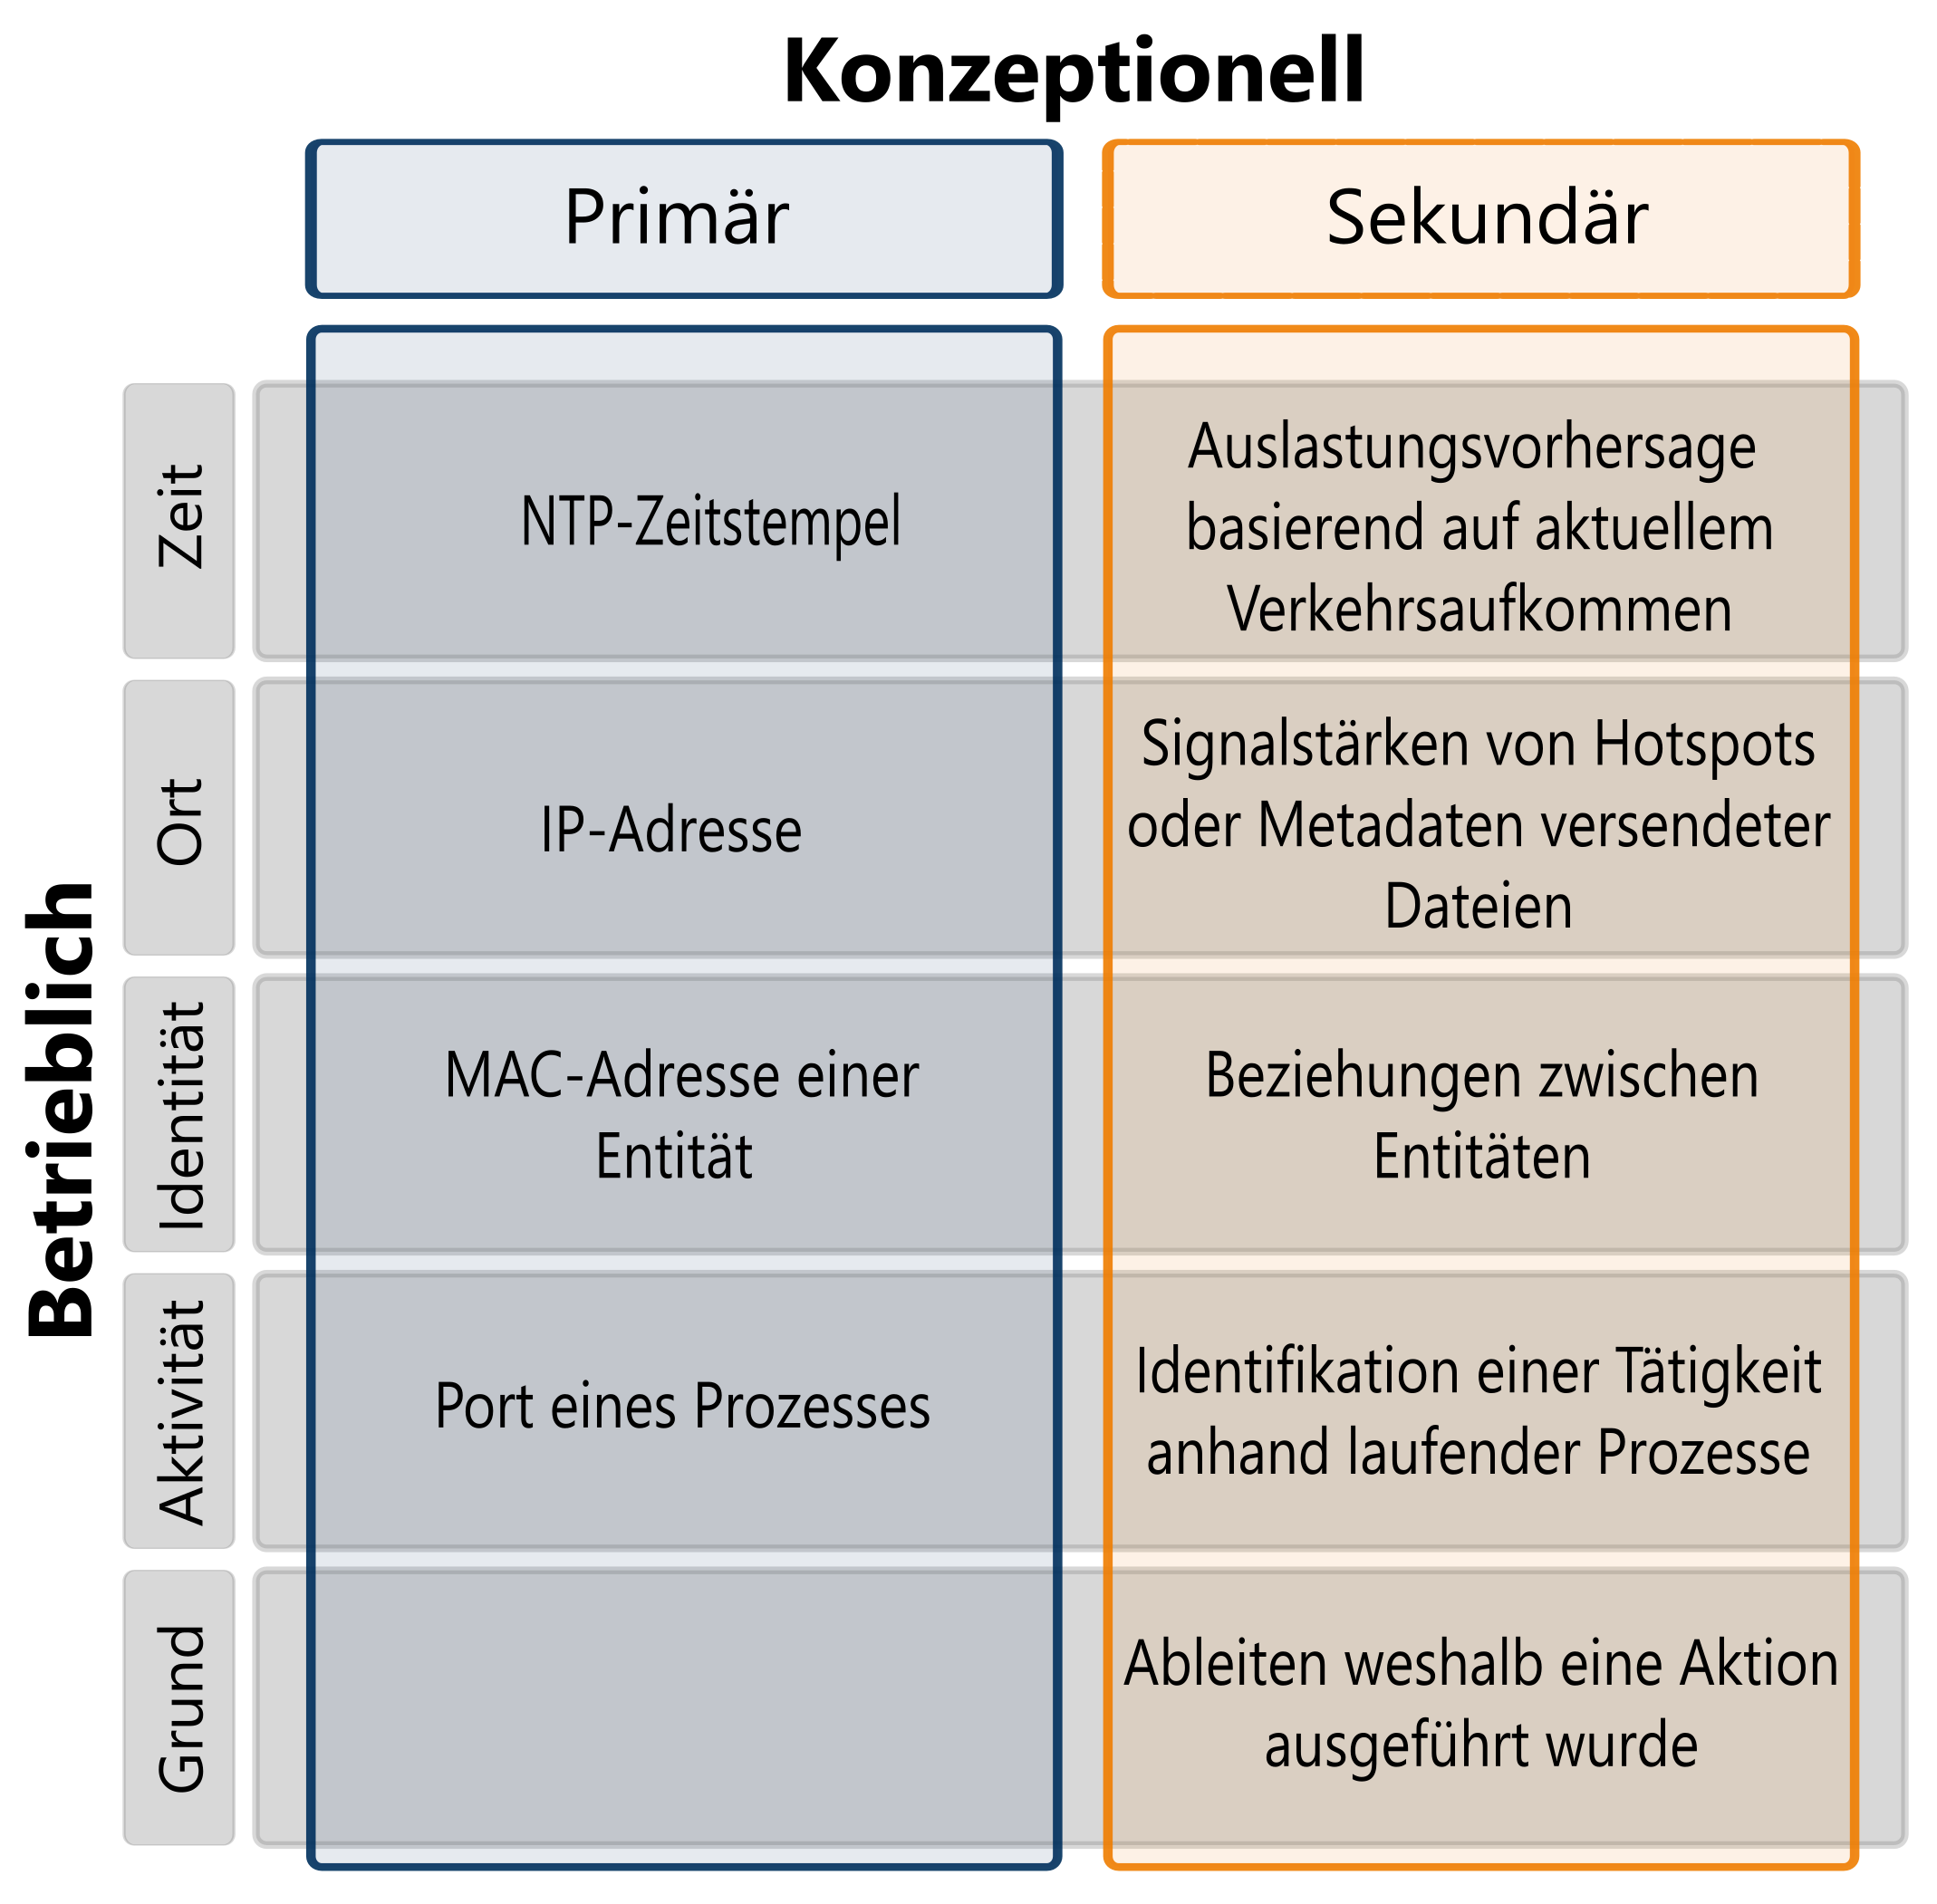
\includegraphics[width=14cm,height=13.5cm]{graphic_1}
%--------------------------
\subsection{Historie}
Die Historie einer Entität wird in dieser Taxonomie zweigeteilt. Sie besteht aus:
\begin{enumerate}
\item{Einem aktiven Teil also ihrem Verhalten, beispielsweise früheren Verbindungen bzw. Verbindungsanfragen}
\item{Einem passiven Teil also dem Zustand der für sie charakteristischen Attribute, beispielsweise einem Nutzernamen oder die Versionsnummer eines bestimmten Programms}
\end{enumerate}
Die Existenz einer Historie trifft die implizite Annahme das eine Entität eindeutig und über einen längeren Zeitraum im Netzwerkverkehr identifizierbar ist.
\subsubsection{Dynamik}
Wie 
 %TODO im Kapitel Hintergrund%
 beschrieben können sich die Werte, aus denen sich die Historie einer Entität zusammensetzt, je nach dem welchem Teil sie zugeordnet werden, verschieden oft ändern.
Statische Messgrößen ändern dabei ihre Werte nie oder nur sehr selten. Dynamische Messgrößen hingegen sehr oft. In diesem Fall wird eine Unterteilung jährlich, monatlich, wöchentlich, täglich, stündlich, minütlich und sekündlich vorgenommen.
\subsubsection{Raten}
Die Historie ist weiterhin in 3 verschiedene Bereiche unterteilt. Abhängig davon wo die Änderung auftritt und ob das IDS oder eine Entität die Aktualisierung des Wertes auslöst.
\paragraph{Änderungsrate} 
Gibt an wie oft eine Entität eine Werteänderungen mitteilt.
\paragraph{Abtastrate}
Wie oft Werte einer Entität vom IDS abgefragt bzw aktualisiert werden.
\paragraph{Abfragerate}
Wie oft Werte im Netzwerk von einer Entität, die nicht das IDS ist, abgefragt werden.\\\\
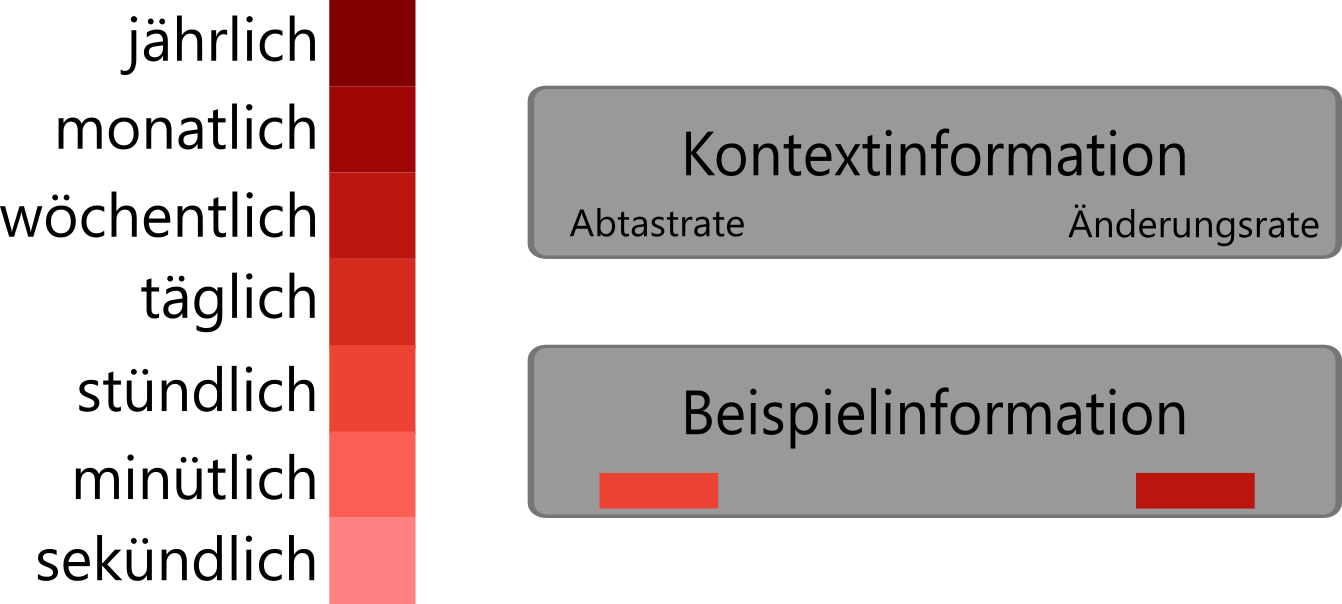
\includegraphics{history}
%--------------------------

\subsection{Logisch}
\subsubsection{Protokoll}
Kategorisierung anhand des verwendeten Kommunikationsprotokolls. Orientiert sich am ISO/OSI-Referenzmodell \cite{day1983osi}. Die Zuordnung zu einer bestimmten Schicht und damit Kategorie erfolgt anhand der für die einzelnen Schichten üblichen Protokolle. Ermöglicht die Identifikation von Entitäten anhand der von ihnen genutzten Protokolle. So kann beispielsweise ein Switch oder Router von einem Nutzer unterschieden werden.
\paragraph{Anwendung}
Beinhaltet allen Netzwerkverkehr der sich der Sitzungsschicht, Darstellungsschicht oder Anwendungsschicht zuordnen lässt 
\paragraph{Transport}
Pakete die sich der Transportschicht zuordnen lassen.
\paragraph{Vermittlung}
Netzwerkverkehr der zur Vermittlungsschicht gehört.


\subsubsection{Attribute der Entitäten}
Kategorisierung von Kontextinformationen abhängig davon welche Art von Entität sie betreffen.
Diese Unterscheidung setzt genauso wie die Historie eindeutig identifizierbare Entitäten voraus.
\paragraph{Gerät}
Informationen die sich auf ein spezifisches Gerät beziehen
\begin{enumerate}
\item{Ein Gerät ist beispielsweise einen Router oder das Endgerät eines Nutzers. }
\item{Informationen können beispielsweise die Liste an installierter Software, die Menge laufender Prozesse oder die Auslastung der Hardwarekomponenten sein.}
\end{enumerate}
\paragraph{Nutzer}
Informationen die sich auf einen Nutzer beziehen.
\begin{enumerate}
\item{Ein Nutzer im Sinne eines Computersystems und keine physische Person. So kann eine physische Person durchaus mehrere verschiedene logische Nutzerkonten haben. }
\item{Informationen können zum Beispiel die Zugriffsrechte eines Nutzers sein.}
\end{enumerate}
\paragraph{Anwendung}
Informationen die sich auf eine Anwendung beziehen.
\begin{enumerate}
\item{Anwendung umfasst jegliche Softwareprozesse die für sich oder in Kombination einen bestimmten Zweck erfüllen.}
\item{Eine Anwendung erzeugt für sie charakteristischen Netzwerkverkehr, versendet oder empfängt also bestimmte Informationen.}
\end{enumerate}
\subsection{Verhaltensbezogen}
Einordnung der Kontextinformationen abhängig davon sie der für den Anwendungsfall definierten Normen entsprechen.
\subsubsection{Erwartetes Verhalten}
Werte der Kategorien oder Verhalten von Entitäten passend  zu den im Netzwerk vorherrschenden Bedingungen.
\subsubsection{ungewöhnliches Verhalten}
Werte der Kategorien oder Verhalten von Entitäten die in Kombination mit den im Netzwerk vorherrschenden Bedingungen entweder auffällig oder irrational sind.

\newpage
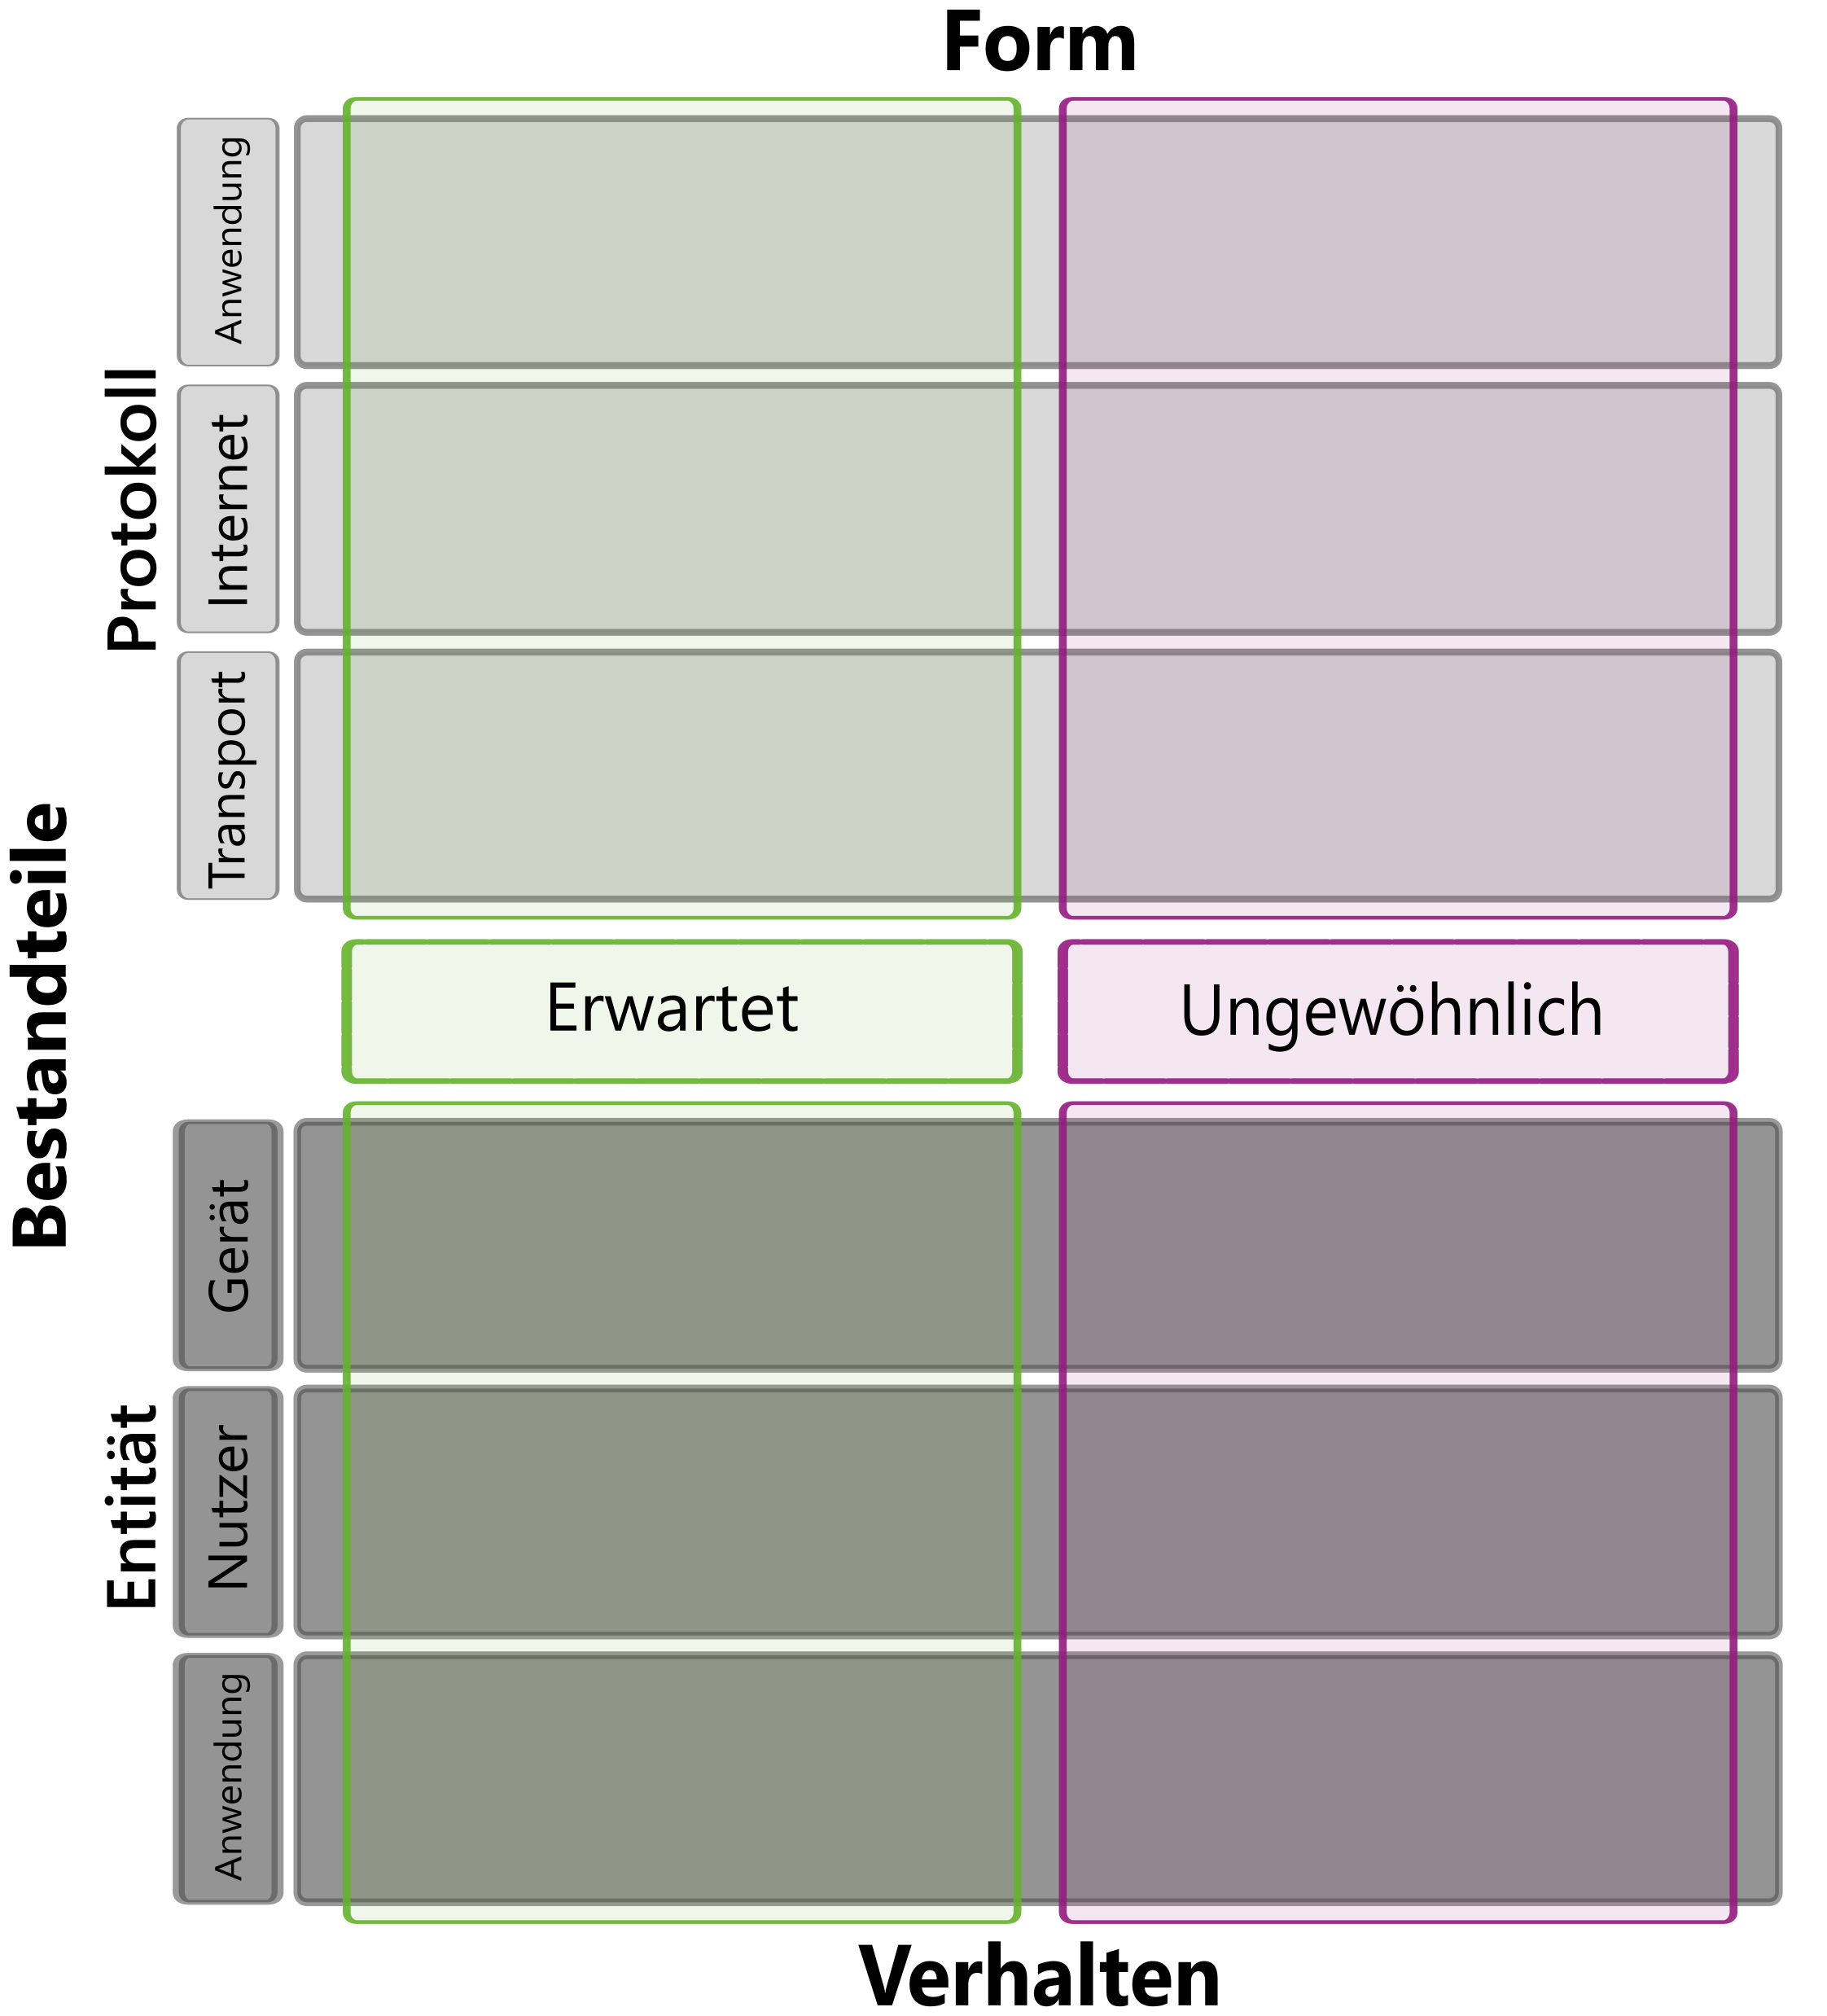
\includegraphics[width=15cm,height=17.5cm]{graphic_2}
\section{Form des Kontextes}
Nachdem die einzelnen Kategorien definiert wurden muss man auch noch festlegen in welcher Form die Kontextinformationen vorliegen sollen bzw. gebracht werden müssen.
%TODO work in Progress

\subsection{Historie}
%Scr-IP/Port + Dest-IP/Port
%Zeitpunkt
%Protokoll
%Paketlänge
%Verbindung möglich
%Verbindung zugelassen
\section{Kontextgewinnung}
%Wo genau bekommt man Kontextinformationen her 
Abschließend muss man die benötigten Kontextinformationen noch sammeln.
Dabei sollte man bedenken an welcher Stelle und wie oft man Informationen abruft oder automatisch aktualisiert. \cite{perera_context_2014}

  Es folgt eine Übersicht einiger Möglichkeiten Kontext zu gewinnen.    
%TODO  A Context Aware Network-IDS
- osquery
- network (open ports) | Nessus
- devices in network | Configuration Management Database (CMDB), nmap   
- cve reference - yes/no
- protocol header


	

\section{Umwandlung der Taxonomie in IDS-Signaturen} 

%What is important for the reader is to understand that the contextual awareness of machines is from a radically different nature than the one of humans. Also, that computational systems are good at gathering and aggregating data, but humans are still better at recognizing contexts and determining what action is appropriate in a certain situation [2]. On the other hand, positivism looks at context as a representational problem, considering it as a “form of information, delineable, stable and separable from activity” [5]. The definitions made in the context-aware field, naturally adopt this point of view. For instance, Dey’s definition [10] allows designers to use the concept for determining why a situation occurs and use this to encode some action in the application [26], making the concept operational in terms of the actors and information sources [17]. Nevertheless, since the definition inherently has a positivist view, the potential of C-AS remains limited to the context that developers are able to encode and foresee. \cite{alegre_engineering_2016}
Um die im Abschnitt Kontexttaxionomie festgelegten Kategorien in Signaturen für ein Intrusion Detection System umzuwandeln zu können gilt es gewisse Dinge zu beachten:\\\\ Die Kontextsensitivität eines Computers unterscheidet sich drastisch von der eines Menschen. Rechensysteme sind sehr gut darin Daten zu erfassen und zu sammeln, aber Menschen sind immer-noch nötig um verschiedene Kontexte zu erkennen und zu entscheiden welches Handeln in einer bestimmten Situation angemessen ist \cite{dey_understanding_2001}.\\
Der limitierende Faktor des Potenzials eines kontextsensitiven Systems ist das Maß an Kontext das ein Entwickler vorhersehen und kodieren kann.\\
%The list of unforeseen or undetectable contexts can be endless.Summarizing, if developers can not determine all that can be affected by an action, it will be very difficult to write a closed and comprehensive set of actions to take in those cases.
Es ist aber weder beim Design noch später bei der Implementierung unmöglich alle Zusammenhänge vorherzusehen.\\
Dementsprechend schwer wird ist es ein in sich geschlossenes und allumfassendes Regelset festzulegen \cite{perera_context_2014}.\\\\
%“(A) Enumerate the set of contextual states that may exist;” 
%“(B) Know what information could accurately determine a contextual state within that set;” 
%“(C) State what appropriate action should be taken in a particular state.”
 Nach Greenberg et al. \cite{greenberg2001context} gibt 3 non-triviale Hauptaspekte die man beim Entwerfen eines kontextsensitiven Systems beachten sollte: 
%Mehr erklärung nötig?
\begin{enumerate}
\item{Spezifizieren aller möglichen Kontextzustände}
\item{Wissen welche Informationen einen konkreten Kontextzustand akkurat festlegen.}
\item{Welche Aktion im jeweiligen Zustand ausgeführt werden sollen.}
\end{enumerate}

\subsection{Entscheidung für ein IDS}
IDSs können anhand der überwachten Plattform, der verwendeten Erkennungsmethode und der Struktur in der sie eingesetzt werden kategorisiert werden.


\begin{tabularx}{\columnwidth}{l|l|l}
\hline
Eigenschaft & IDS Typ & Beschreibung\\
\hline
Plattform   & Host     & Überwacht Aktivitäten auf dem System auf dem es eingesetzt wird um lokale Angriffe zu erkennen. \\
& Netzwerk & Überwacht Aktivitäten im Netzwerk um Angriffe, die über eine Netzwerkverbindung ausgeführt werden zu erkennen.\\ 
& Hybrid   & Kombiniert host- und netzwerk-basierte Intrusion Detection Systeme.\\
\hline
Angriffserkennung & Signatur        & \\
                  & Anomalie        & \\
                  & Hybrid          & \\ 
\hline
\end{tabularx}

%TODO NIDS vs HIDS + signature vs anomaly -> zeek+osquery
\subsection{Verbesserung der Schwächen des gewählten IDS}
Zuerst einmal stellt sich die Frage: Wie einfach lassen sich die Zustände die auftretender Kontext annehmen kann in Regeln festlegen? Der Nachteil eines rein signatur-basierten IDS ausschließlich Angriffe zu erkennen die vordefinierten Verhaltensmustern entsprechen will ich verbessern. Dazu verwende ich das bereits erwähnte "osquery" um die Signatur
\subsection{ Vergleich der Taxonomie und der zur Verfügung stehenden Informationen}
Die Informationen die ich in den definierten Kategorien als gegeben vorausgesetzt habe sind in der Praxis unterschiedlich schwer zu akquirieren. Offensichtlich ist es um ein Vielfaches einfacher korrekt die aktuelle Uhrzeit zu ermitteln als den Grund dafür das ein Nutzer eine Aktion ausführt zu bestimmen. Die nachfolgende Grafik dient dazu den meiner Einschätzung nach benötigten Aufwand zur Beschaffung einer Information zu veranschaulichen.
%TODO Grafik
\section{Anspruch an das IDS}
Um die Performance des gewählten IDS verbessern zu können, muss man festlegen welche Kriterien die Leistung beeinflussen bzw. bestimmen.
Mell et al.\cite{mell2003overview} nennen in ihrer Übersicht verschiedene Charakteristiken zur quantitativen Bestimmung der Erkennungsgenauigkeit eines IDS und erläutern zusätzlich die Wechselwirkungen zwischen einzelnen Kriterien, die beim Vergleich verschiedener IDS-Lösungen beachtet werden sollten.
%Coverage: This measurement determines which attacks an IDS can detect under ideal conditions. 
\subsubsection{Abdeckung}
Gibt an welche Typen von Angriffen ein IDS unter idealen Bedingungen feststellen kann.
% Probability of False Alarms 
%This measurement determines the rate of false positives produced by an IDS in a given environment during a particular time frame. A false positive or false alarm is an alert caused by normal non- malicious background traffic
\subsubsection{Wahrscheinlichkeit falscher Alarme}
Gibt die Wahrscheinlichkeit das durch ein IDS ausgelöste Alarme durch gutartigen bzw. nicht-schädlichen Netzwerkverkehr verursacht wurden an.\\
\[Rate\;an\;falsch-Positiven\;Meldungen = \frac{Anzahl\;falscher\;Alarme}{Anzahl\;aller\;Alarme}\]
%Probability of Detection: 
%This measurement determines the rate of attacks detected correctly by an IDS in a given environment during a particular time frame
\subsubsection{Wahrscheinlichkeit einer Erkennung}
Gibt die Rate der durch das IDS korrekt erkannten Angriffe an.\\
\[Erkennungswarscheinlichkeit  = \frac{Anzahl\;korrekt\;erkannter\;Angriffe} {Anzahl\;aller\;Angriffe}\]
%Resistance to Attacks Directed at the IDS This measurement demonstrates how resistant an IDS is to an attacker's attempt to disrupt the correct operation of the IDS. Attacks against an IDS may take the form of: 
%1. Sending a large amount of non-attack traffic with volume exceeding the IDS’s processing capability. With too much traffic to process, an IDS may drop packets and be unable to detect attacks. 
%2. Sending to the IDS non-attack packets that are specially crafted to trigger many signatures within the IDS, thereby overwhelming the IDS’s human operator with false positives or crashing alert processing or display tools. 
%3. Sending to the IDS a large number of attack packets intended to distract the IDS’s human operator while the attacker instigates a real attack
\subsubsection{Resistenz}
Ein signatur-basiertes IDS bzw. der menschliche Administrator hinter dem System weisen Probleme auf die nicht direkt beim Umgang mit verarbeitetem Netzwerkverkehr, sondern schon bei der bewussten, unbewussten, oder erzwungenen Entscheidung welcher Netzwerkverkehr überhaupt in Frage kommt, entstehen:
\begin{enumerate}
\item{Ein zu große Menge an zu verarbeitendem Netzwerkverkehr die die Verarbeitungskapazität eines IDS übersteigt kann dazu führen das Netzwerkpakete verworfen und Angriffe nicht erkannt werden}
\item{Pakete die zwar nicht bösartig sind aber so konstruiert das sie möglichst viele IDS Signaturen auslösen, überfordern den Administrator oder stören eventuell sogar die Verarbeitung von Paketen generell. }
\item{Ein Angreifer könnte eine Vielzahl "harmloserer" aber trotzdem noch als schädlich zu deklarierende Pakete senden um einen größeren Angriff im Netzwerkverkehr zu verschleiern.}
\item{Pakete die möglicherweise vorhandene Fehler im IDS selbst ausnutzen.}
\end{enumerate}
%Ability to Correlate Events: This measurement demonstrates how well an IDS correlates attack events. These events may be gathered from IDSs, routers, firewalls, application logs, or a wide variety of other devices.
\subsubsection{Korrelation zwischen Einzelereignissen }
Demonstriert wie gut ein IDS eine Korrelation zwischen einzelnen Ereignissen, möglicherweise verschiedenen Ursprungs herzustellen. Die Ereignisse können dabei aus Routern, Firewalls, Anwendungen, dem IDS selbst oder einer großen Bandbreite anderer Quellen stammen.
%Ability to Detect Never Before Seen Attacks: This measurement demonstrates how well an IDS can detect attacks that have not occurred before. For commercial systems, it is generally not useful to take this measurement since their signature-based technology can only detect attacks that had occurred previously (with a few exceptions). However, research systems based on anomaly detection or specification-based approaches may be suitable for this type of measurement. Usually systems detecting attacks that had never been detected before produce more false positives than those that do not have this feature.
\subsubsection{Unbekannte Angriffe vorhersehen}
Gibt an wie gut ein IDS einen Angriff erkennt der so noch nicht aufgetreten ist. Signatur-basierte IDS sind allgemein, mit wenigen Ausnahmen, nicht in der Lage solch einen Angriff zu erkennen. Normalerweise erhöht die Fähigkeit eines Systems einen noch unbekannten Angriff zu erkennen, im Vergleich zu Systemen die dies nicht versuchen, zusätzlich die Rate an falsch-positiven Meldungen.
%Ability to Identify an Attack: This measurement demonstrates how well an IDS can identify the attack that it has detected by labeling each attack with a common name or vulnerability name or by assigning the attack to a category.
\subsubsection{Identifizieren von Angriffen}
Wie gut ein IDS einem Angriff den es erkennt, einen Namen oder eine Kategorie, beispielsweise ein CVE-Nummer, zuordnen kann.
%Ability to Determine Attack Success: This measurement demonstrates if the IDS can determine the success of attacks from remote sites that give the attacker higher- level privileges on the attacked system. In current network environments, many remote privilege-gaining attacks (or probes) fail and do not damage the system attacked. Many IDSs, however, do not distinguish the failed from the successful attacks. For the same attack, some IDSs can detect the evidence of damages (whether the attack has succeeded) and some IDSs detect only the signature of attack actions (with no indication whether the attack succeeded or not). The ability to determine attack success is essential for the analysis of the attack correlation and the attack scenario; it also greatly simplifies an analyst’s work by distinguishing between more important successful attacks and the usually less damaging failed attacks. Measuring this capability requires the information about failed attacks as well as successful attacks.
\subsubsection{Beurteilung  eines Angriffs}
Indikator dafür ob ein IDS den Erfolg und die Auswirkungen eines Angriffes korrekt beurteilen kann. In aktuellen Netzwerkumgebungen schlagen viele Angriffs(-vesuche) fehl. Die meisten IDS unterscheiden allerdings nicht zwischen erfolgreichen und fehlgeschlagenen Angriffen. Für den selben Angriff können manche IDS die Anzeichen dafür ob ein Angriff erfolgreich war erkennen, andere lediglich das ein Angriff stattgefunden hat, allerdings ohne feststellen zu können ob er erfolgreich war. Die Fähigkeit, den Grad zu dem ein Angriff auf das überwachte System erfolgreich war zu beurteilen ist essenziell. Eine Vorfilterung der Meldungen durch das IDS vereinfacht die Arbeit des Netzwerkadministrators bzw. Analysten stark, da so eine Analyse des Angriffsszenarios und der Korrelation einzelner Angriffe vereinfacht wird. Diese Fähigkeit bei einem gegebenen IDS messen zu können setzt das Wissen, darüber welche Angriffe erfolgreich sind und welche nicht, voraus.

% Other Measurements
% There are other measurements, such as ease of use, ease of maintenance, deployments issues, resource requirements, availability and quality of support etc. These measurements are not directly related to the IDS performance but may be more significant

\subsection{Einordnung der Kriterien}
% Also, the probability of detection varies with the false positive rate, and an IDS can be configured or tuned to favor either the ability to detect attacks or to minimize false positives
%TODO weiter erklären
Die Wahrscheinlichkeit einen Angriff zu erkennen variiert mit der Rate an falsch-positiven Meldungen. Bei der Konfiguration eines IDS kann entweder die Falsch-positiv-Rate oder die Erkennungsrate optimiert werden.

%unterscheidung performance/security related metrics 
\subsection{Auswahl der Kriterien}
\cite{milenkoski_evaluating_2015}
In dieser Arbeit beschäftige ich mich ausschließlich mit sicherheitsrelevanten Leistungsmetriken. Dabei will ich hauptsächlich den Einfluss von Kontextsensitivtät auf die Abdeckung, die Erkennungswahrscheinlichkeit, die Wahrscheinlichkeit  falscher Alarme und die Interpretierbarkeit von Meldungen durch einen menschlichen Nutzer betrachten. Zusätzlich will ich beleuchten inwiefern Kontext die Korrelation zwischen Einzelereignissen und das Identifizieren von Angriffen ermöglicht bzw. verbessert.
%One of the primary goals of this correlation is to identify staged penetration attacks. Currently, IDSs have only limited capabilities in this area.
%Überleitung  zu CAAC
\section{Kontextsensitivität}
\chapter{Implementierung}%
\label{cha:implementation}

%In this chapter, you should provide technical details on how you actually implemented the design that you derived in the previous chapter.

% Comparative study and analysis of network intrusion detection tools

%\subsection{ Umsetzung/Implementierung der Taxonomie in  IDS-Signaturen}
%\section{Test der kontextsensitiven Signaturen}

%\subsection{ (Auswahl eines bereits existierenden/ Erstellung eines eigenen) Datensatzes + dazugehörige Label }
%\subsection{ Aufbau eines oder mehrerer Netzwerke  } 
%\subsection{ Setup der verschiedenen IDS }
%\subsection{ Grundlage mit non-kontextsensitiven Signaturen auf Datensatz}
%\subsection{ Test der kontextsensitiven Signaturen auf Datensatz} 

Der im Kapitel \ref{cha:design} dargelegte Aufbau eines Netzwerkes findet sich auch in der Implementation wieder. Scapy, Wireshark und Zeek verarbeiten Kommunikationsdaten, Zeek-agent stellt die Attribute der Entitäten bereit und mit den Skripten werden die geltenden Normen und das dadurch abgedeckte Verhalten festgelegt.
\section{Erläuterung der wichtigsten Komponenten}
Eine kurze Vorstellung der wichtigsten Komponenten der Implementierung, insofern sie im Rahmen der einzelnen Schritte des Versuchsaufbaus essenziell sind.
\subsection{Zeek}
%TODO
%Zeek is a passive, open-source network traffic analyzer. Many operators use Zeek as a network security monitor (NSM) to support investigations of suspicious or malicious activity.
%Zeek is a fully customizable and extensible platform for traffic analysis. Zeek provides users a domain-specific, Turing-complete scripting language for expressing arbitrary analysis tasks
%In brief, Zeek is optimized for interpreting network traffic and generating logs based on that traffic. It is not optimized for byte matching, and users seeking signature detection approaches would be better served by trying intrusion detection systems such as Suricata. Zeek is also not a protocol analyzer in the sense of Wireshark, seeking to depict every element of network traffic at the frame level, or a system for storing traffic in packet capture (PCAP) form. Rather, Zeek sits at the “happy medium” representing compact yet high fidelity network logs, generating better understanding of network traffic and usage.
%Zeek as a NSM platform enables collection of at least two, and in some ways three, of these data forms, namely transaction data, extracted content, and alert data
Ein passives, quelloffenes Analysewerkzeug für Netzwerkverkehr, das durch eine eigene Skriptsprache unter anderem die Implementierung beliebiger Analyseaufgaben, die Interpretation von Netzwerkverkehr und Erstellung von Protokollen auf der Grundlage dieses Verkehrs ermöglicht.\\
Zeek ist dabei weder rein signatur-basiert wie Suricata noch ausschließlich als Protokollanalysator im Sinne von Wireshark zu verstehen. Vielmehr handelt es sich bei Zeek um eine Mischung, die eine kompakte, aber dennoch detailgetreue Darstellung von Netzwerkprotokollen ermöglicht. Dies erlaubt ein besseres Verständnis des Netzwerkverkehrs und der Netzwerknutzung \cite{zeek_about_page}.

\subsection{Zeek-Agent}
Zeek-Agent ist ein Endpunkt-Agent, der Informationen für zentrales Monitoring an Zeek sendet.
Abfragen kann man verschiedene Aktivitäten eines Hostsystems, darunter zum Beispiel aktuell laufende Prozesse, offene Sockets oder den Inhalt bestimmter Dateien. Diese erscheinen in Zeek, genauso wie Netzwerkaktivität als Ereignisse und können so in Skripten verwendet werden \cite{zeek_agent}.

\section{Versuchsaufbau}
Der Ablauf für alle Anwendungsfälle ist grundsätzlich sehr ähnlich:
\begin{enumerate}
%\item{Spezifikation des Netzwerkes}
\item{Erzeugung}
\item{Mitschnitt via WireShark}
\item{Analyse mittels Zeek und Zeek-Agent}
\begin{enumerate}
\item{Einlesen von Netzwerkverkehr}
\item{Einbindung des zusätzlichen Kontextes}
\item{Logging}
\end{enumerate}
\end{enumerate}
\subsection{Erzeugung}
%\subsubsection{Scapy}
Der Netzwerkverkehr wurde mit Hilfe von Scapy generiert. Das ermöglicht den für die verschiedenen Szenarien benötigten Netzwerkverkehr zu erzeugen und die einzelnen Schichten eines Pakets an den jeweiligen Anwendungsfall anzupassen. In Abbildung \ref{scapy} ist dieser Prozess ausschnittsweise dargestellt. Eine Übersicht über alle dafür verwendeten Skripte findet sich im Anhang.
\begin{lstlisting}[label={scapy},language=python,caption={Konfiguration und Versendung eines Pakets},firstnumber=6]
def send_packet(ip_address_src,ip_address_dst):
    source_server = ip_address_src
    target_server = ip_address_dst
    layer_2 = Ether()
    layer_3 = IP(src=source_server, dst=target_server)
    layer_4 = TCP(sport=80,dport=43468)
    tcp_pkt = layer_2 / layer_3 / layer_4
    sendp(tcp_pkt)
\end{lstlisting}

%\subsection{Mitschnitt}
%\subsubsection{Wireshark}
%Der Mitschitt der von Scapy versendeten Pakets erfolgt mit Wireshark. Die mitgeschnittenen Pakets werden im als pcap-Dateien gespeichert um das einlesen in Zeek zu ermöglichen.


%defining the format of your data, letting Zeek know that you wish to create a new log, and then calling the Log::write method to output log records.
\subsection{Logging}
In Zeek erfolgt das Schreiben in Logs immer nach demselben Prinzip:
\begin{enumerate}
\item{Vor dem Ausführen eines Skriptes wird ein Log und die darin zu speichernden Informationen festgelegt (Z. \ref{logging_1}-\ref{logging_2})}
\item{Nutzer-definierter Log wird initialisiert (Z. \ref{logging_3})}
\item{Form des Eintrags für den Log wird definiert (Z. \ref{logging_4})}
\item{Log-Eintrag wird der Verbindung als Information hinzugefügt (Z. \ref{logging_5})}
\item{Eintrag wird in Log geschrieben (Z. \ref{logging_6})}
\end{enumerate}
\lstset{escapeinside={(*@}{@*)}}
\begin{lstlisting}[consecutivenumbers=false,numberblanklines=false,caption={Generierung einer Log-Datei mit Verbindungsinformationen},label={Code_2}]
export {
    # Create an ID for our new stream. By convention, this is called "LOG".
    redef enum Log::ID += { LOG }; (*@\label{logging_1}@*)	

    # Define the record type that will contain the data to log.
    type Info: record {
        timestamp: time		&log;
        id: connection_id	&log; 
        notice: string		&log;
    };(*@\label{logging_2}@*)
}

redef record connection += {
    # By convention, the name of this new field is the lowercase name
    # of the module.
    examplelog: Info &optional;
};
event zeek_init(){
	Log::create_stream(ExampleModule::LOG, $columns=Info, $path="examplemodule"]);(*@\label{logging_3}@*)
	local record: ExampleLog::Info = $ts=current_time(), $id=c$id, $notice="Example Notice"];(*@\label{logging_4}@*)
    # Store a copy of the data in the connection record so other
    # event handlers can access it.
    c$examplelog = record;(*@\label{logging_5}@*)
    Log::write(ExampleModule::LOG, rec);(*@\label{logging_6}@*)
}
\end{lstlisting}
\section{Skripte}
Der Kern der Implementierung sind Zeek Skripte. Hier werden die gesammelten Kontextinformationen verwendet. Nachfolgend werden für einige ausgewählte Kategorien Anwendungsfälle vorgestellt.
\subsection{Geografische Koordinaten und Ortszeit}
Das Volumen von durch Menschen verursachten Netzwerkverkehr ist in der Regel größtenteils tageszeitabhängig. So wird üblicherweise nachts weniger kommuniziert als am Tag. Deshalb erscheint es sinnvoll, den Grenzwert für erzeugtes Verkehrsaufkommen, ab dem ein Sender als potenziell böswillig eingestuft wird, je nach Uhrzeit anzupassen. \\

Das Skript ordnet eine IP-Adresse zu einem geografischen Ort zu (Z. \ref{g_lookup_1}).\\

Berechnet die Ortszeit am Ursprung der Anfrage mithilfe der lokalen Uhrzeit in

Kombination mit dem aus dem Abstand ermittelten Zeitunterschied (Z. \ref{g_lookup_2} - \ref{g_lookup_3}).\\

Passt des Grenzwertes entsprechend an (Z. \ref{g_lookup_4}).\\\pagebreak
\lstset{escapeinside={(*@}{@*)}}
\begin{lstlisting}[consecutivenumbers=false,numberblanklines=false,label={Code_3},caption={Geolokalisierung und Setzen des Grenzwertes},firstnumber=31,linerange={31-37,42-54}]
module GeoLogTest;

export {
    # Create an ID for our new stream. By convention, this is called "LOG".
    redef enum Log::ID += { LOG };

    # Define the record type that will contain the data to log.
    type Info: record {
        ts: time        &log;
        rts : string 	&log;
        id: conn_id     &log; 
        notice : string &log;
    };
}

redef record connection += {
    # By convention, the name of this new field is the lowercase name of the module.
    geologtest: Info &optional;
};

global ip_addresses : tableaddr] of int;
global threshold : int; 
global night_time_decrease : int;
global day_time_increase : int;
#const home_country = "DE";
#const home_latitude = 51.025889;
const home_longitude = 13.723376;
const closing_time = 19;
const opening_time = 7;

function geolocation(c: connection):double{
	local origin_longitude = lookup_location(c$id$orig_h)$longitude;(*@\label{g_lookup_1}@*)
	return origin_longitude;
}

function time_at_geolocation(longitude: double): int{ (*@\label{g_lookup_2}@*)
	local time_to_add  = (longitude - home_longitude)*240;
	local time_difference = network_time()) + time_to_add;
	local epoch_time_difference = double_to_time(epoch_time_difference);
	local time_at_origin  = strftime("%H", epoch_time_difference);
	local useable_time_at_origin = to_int(time_at_origin);
	return useable_time_at_origin; (*@\label{g_lookup_3}@*)
}

function set_threshold(c_time: int): double{ (*@\label{g_lookup_4}@*)
	if(c_time< opening_time || c_time > closing_time )
		threshold = threshold-night_time_decrease;
	else 
		threshold = threshold+day_time_increase;
	return threshold; 
}
\end{lstlisting}
%\begin{figure}H]

%\caption{Setzen des Grenzwertes von Verbindungsversuchen}
%\end{figure}
\subsection{Verwendete Ports}
%Verwendet werden Ports die die aktuell auf dem System laufenden Prozesse.
Wenn eine Verbindung oder ein Verbindungsversuch mit einem bestimmten Port des Systems als Ziel beobachtet wird, ohne das es einen Prozess gibt, der diesem Port durch Zeek-Agent zugeordnet werden kann, wird die Verbindung oder der Verbindungsversuch im dazugehörigen Log vermerkt.\\

Das Skript erfragt bei den Instanzen des Zeek-Agents in regelmäßigen Abständen die auf

Hostsystemen laufenden Prozesse und deren verwendete Ports (Z. \ref{p_lookup_1} und \ref{p_lookup_1_2}).\\

Das Skript vergleicht den Zielport jeder eingehenden Verbindung mit der Liste von 

verwendeten Ports auf dem Hostsystem (Z. \ref{p_lookup_2}).\\

Abhängig vom Ergebnis wird eine Meldung in den Log geschrieben (Z. \ref{p_lookup_3}).
\begin{lstlisting}[caption={Abfrage und Abgleich der Ports },label={Code_4},consecutivenumbers=false,lastline=77,firstnumber=52,numberblanklines=false,linerange={52-55,62-70,76-77}]
@load site/packages/zeek-agent-v2
@load site/packages/zeek-agent-v2/framework/main
@load site/packages/zeek-agent-v2/table
@load site/zeek-agent-v2
@load site/zeek-agent-v2/framework
@load site/zeek-agent-v2/table


module Querytest;

export {
    # Create an ID for our new stream. By convention, this is
    # called "LOG".
    redef enum Log::ID += { LOG };

    # Define the record type that will contain the data to log.
    type Info: record {
        ts: time        &log;
        id: conn_id     &log; 
        notice : string &log;
    };
}

redef record connection += {
    # By convention, the name of this new field is the lowercase name
    # of the module.
    querytest: Info &optional;
};

type Columns: record {
    name: string &optional &log; ##< short name
    is_admin: bool &optional &log; ##< 1 if user has adminstrative privileges
    process: string &optional &log; ##< name of process holding socket
    protocol: count &optional &log; ##< transport protocol
    local_addr: addr &optional &log; ##< local IP address
    local_port: count &optional &log; ##< local port number
    remote_addr: addr &optional &log; ##< remote IP address
    remote_port: count &optional &log; ##< remote port number
};


global local_ports : table[int] of string ={
        [80] = "http",
        [22] = "ssh",
        [25552] = "application_1",
    };
global allowed_ports : table[int] of string = {
        [42124] = "application_2",
        [42125] = "application_3" 
    };

function check_outgoing_connection(c:connection){
    local _port = port_to_count(c$id$orig_p);
    if(_port !in local_ports){{(*@\label{p_lookup_2}@*)
        local rec: Querytest::Info = [$ts=current_time(), $id=c$id, $notice="No Application running on this port"]; (*@\label{p_lookup_3}@*)
    }else{
    	local rec: Querytest::Info = [$ts=current_time(), $id=c$id]}
    # Store a copy of the data in the connection record so other
    # event handlers can access it.
    c$querytest = rec;
    Log::write(Querytest::LOG, rec);}

event users_result(ctx: ZeekAgent::Context, data: Columns) {(*@\label{p_lookup_1_2}@*)
    local new_entry : count;
    local connection_port = data$remote_port;
    new_entry = connection_port;
    local_ports[new_entry] = data$name;
}


event zeek_init(){
	Log::create_stream(Querytest::LOG, [$columns=Info, $path="querytest"]);
    local str_stmt_join = "SELECT users.name, users.is_admin, sockets.process, sockets.protocol, sockets.local_addr, sockets.local_port, sockets.remote_addr, sockets.remote_port FROM users JOIN processes ON users.uid=processes.uid JOIN sockets ON sockets.pid=processes.pid";
    local query_event = users_result;
    local _schedule = 10 secs;
    
    local port_query = ZeekAgent::query([$sql_stmt=str_stmt_join, $event_=query_event, $schedule_=_schedule]);(*@\label{p_lookup_1}@*)


event connection_state_remove(c: connection){
    check_outgoing_connection(c);
}

event zeek_done(){
    print "Done";
}
\end{lstlisting}
\subsection{DNS-Auflösung}
Menschliche Nutzer verwenden bei der Nutzung ihres Endgerätes im Gegensatz zu Computern keine IP-Adressen, um Suchanfragen zu formulieren. DNS ordnet IP-Adressen menschenfreundliche Domainnamen zu. Wenn das System eines Nutzers eine Verbindung aufbaut, geht dem eine DNS-Anfrage von diesem Gerät an einen DNS-Nameserver voraus oder die IP-Adresse ist in lokalen Konfigurationsdateien auffindbar. Wenn beispielsweise eine TCP-Verbindung eines Webbrowsers beobachtet wird, ohne dass eine zuordenbare DNS-Anfrage erfolgt ist oder die IP-Adresse in der Routingdatei des Endgerätes vermerkt ist, ist das in den meisten Fällen ein Grund zum Handeln.\\

Das Skript loggt für jede Antwort eines DNS-Servers die aufgelöste URL und dazugehörige 

IP-Adresse (Z. \ref{dns_lookup_2}).\\

Parallel dazu wird periodisch die Hosts-Datei eines Unix-Systems abgefragt(Z. \ref{dns_lookup_1}).\\

Im Log vermerkt sind ausgehende Verbindungen, deren Zieladressen vorher nicht durch 

einen DNS-Server oder die Hosts-Datei aufgelöst wurden (Z. \ref{dns_lookup_3}).

\begin{lstlisting}[firstnumber=45,consecutivenumbers=false,label={Code_5},linerange={45-45,47-52,58-59,61-64,65-73},caption={Überprüfung der Verbindungsziele eines Endgerätes},numberblanklines=false]
@load site/packages/zeek-agent-v2
@load site/packages/zeek-agent-v2/framework/main
@load site/packages/zeek-agent-v2/table
@load site/zeek-agent-v2
@load site/zeek-agent-v2/framework
@load site/zeek-agent-v2/table
@load base/protocols/conn/contents
@load base/protocols/dns
@load base/bif
module DNStest;

export {
    # Create an ID for our new stream. By convention, this is
    # called "LOG".
    redef enum Log::ID += { LOG };

    # Define the record type that will contain the data to log.
    type Info: record {
        ts: time        &log;
        id: conn_id     &log; 
        notice : string &log;
    };
}   

redef record connection += {
    # By convention, the name of this new field is the lowercase name
    # of the module.
    dnstest: Info &optional;
};

type Columns: record{
    line_content : vector of string &log;
};

global resolved_addresses : table [addr] of string={
    [1.2.3.4] = "www.example.com"
};
global dns_server : set[addr];

event zeek_init(){
    Log::create_stream(DNStest::LOG, [$columns=Info, $path="dnstest"]);
}

#An event that can be handled to access the DNS::Info record as it is sent to the logging framework.
event DNS::log_dns(rec:DNS::Info){
    # builds pair of ip addr that gets send to name-server and the resolved answer string
    local query : string = rec$query;
    local answer : vector of string = rec$answers;
    local answer_address  = to_addr(answer[1]);
    resolved_addresses [answer_address] = query; (*@\label{dns_lookup_2}@*)
}

event query_result(ctx: ZeekAgent::Context, data: Columns){
    local ip_address = to_addr(data$line_content[0]);
    local host_name = data$line_content[1];
    resolved_addresses[ip_address] = host_name + " from local hosts";
}

function query_hosts_file(){
    local str_stmt_hosts = "SELECT columns FROM files_columns(\"/etc/hosts\",\"$1:text,$2:text\")";
    local query_event = query_result;
    local _schedule =  30 secs;
    local hosts_file_query = ZeekAgent::query([$sql_stmt=str_stmt_hosts, $event_=query_event, $schedule_=_schedule]);(*@\label{dns_lookup_1}@*)   
}

event check_resolve_table(c : connection){
    local destination_ip = c$id$resp_h;
    if(destination_ip !in resolved_addresses && destination_ip !in dns_server){ (*@\label{dns_lookup_3}@*)
        local rec: DNStest::Info = [$ts=current_time(), $id=c$id, $notice="Connection without Resolve!"];
        c$dnstest = rec;
        Log::write(DNStest::LOG, rec);
    }
}

# Generated when a connections internal state is about to be removed from memory.
# Zeek generates this event reliably once for every connection when it is about to delete the internal state.
event connection_state_remove(c: connection){
    query_hosts_file();
    local destination_ip = c$id$resp_h;
    local conn_service = c$service;
    # Add DNS-Server to set
    if("DNS" in conn_service){
        add dns_server[destination_ip];
    }
    # schedule resolve check so query result get added to the table before the connection gets checked 
    schedule 45 secs {check_resolve_table(c)}; 
}

# Generated at Zeek termination time.
event zeek_done(){
    print "Done";
}
\end{lstlisting}


\chapter{Evaluation}%
\label{cha:evaluation}

This chapter is usually expected to present which experiments you did as part of your thesis, what results came out of them and what these results tell us about to which extent your design improves the state of the art with regards to the requirements specified in chapter
As a rough outline, this chapter should address the following questions:

\section{Auswertung der Testergebnisse}
\section{ Vergleich der IDS-Alerts mit Datensatzlabeln}
\subsection{ Baselineauswertung } 
\subsection{ Vergleich der Performance gemäß der in 1.1 festgelegten Kriterien zwischen non-kontextsenitiven und kontextsenitiven Signaturen} 
\subsection{ Vergleich der unterschiedlichen getesteten Kontextkategorie(kombinationen)} 

\section{ “Bewertung” der theoretischen Mächtigkeit einzelner Kategorien} 
\section{ Beurteilung/Einschätzung der tatsächlichen Verfügbarkeit von Kontext im Netzwerk }


\section{ Urteil/""Ranking"" der Kontextarten hinsichtlich der Erhöhung der Netzwerksicherheit}


\chapter{Konklusion/Schlussfolgerung}%
\label{cha:conclusion}

%In this chapter, you summarize the conclusions that can be drawn from your thesis with regards to solving the problem explained in the introduction section.
%Furthermore, you should concisely explain further experiments or design options that may be interesting to pursue in future work.


\printbibliography



\end{document}